\documentclass[border=6pt]{standalone}
\usepackage{xcolor}
\definecolor{oiblue}{HTML}{0072B2}
\definecolor{oiorange}{HTML}{E69F00}
\definecolor{oiskyblue}{HTML}{56B4E9}
\definecolor{oigray}{HTML}{999999}
\definecolor{oivermillion}{HTML}{D55E00}
\definecolor{oigreen}{HTML}{009E73}
\definecolor{oipurple}{HTML}{CC79A7}
\usepackage{tikz}
\usepackage{pgfplots}
\pgfplotsset{compat=1.18}
\usepgfplotslibrary{fillbetween}
\usetikzlibrary{shapes,arrows,positioning,calc,patterns,decorations.pathreplacing}
\newcommand{\emrhn}{EMR-HyperNEAT}
\begin{document}
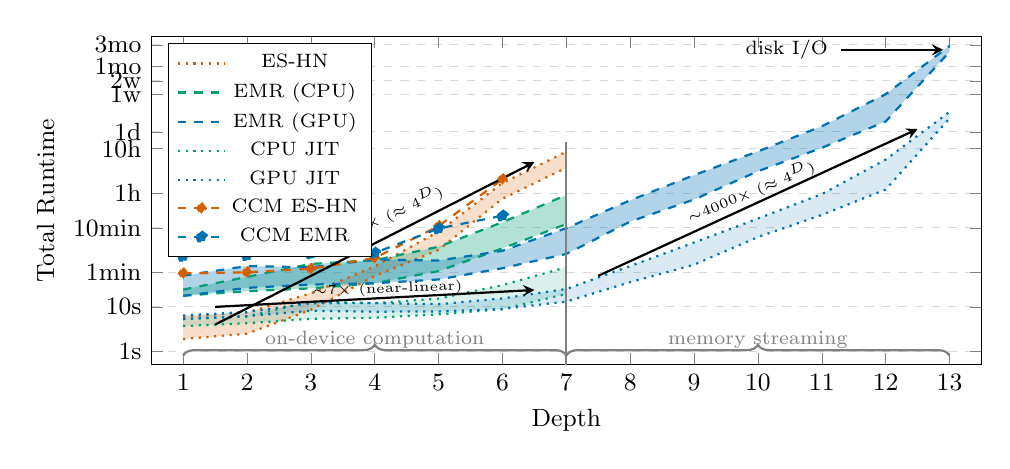
\begin{tikzpicture}
\begin{axis}[
    width=\textwidth,
    height=5.75cm,
    ylabel={Total Runtime},
    xlabel={Depth},
    ymode=log,
    ytick={1, 10, 60, 600, 3600, 36000, 86400, 604800, 1209600, 2592000, 7776000},
    yticklabels={1s, 10s, 1min, 10min, 1h, 10h, 1d, 1w, 2w, 1mo, 3mo},
    ymin=0.5,
    ymax=12000000,
    xmin=0.5,
    xmax=13.5,
    xtick={1,2,3,4,5,6,7,8,9,10,11,12,13},
    xticklabels={1,2,3,4,5,6,7,8,9,10,11,12,13},
    ymajorgrids=true,
    grid style={dashed, gray!30},
    tick label style={font=\small},
    label style={font=\small},
    legend style={at={(0.02,0.98)}, anchor=north west, font=\scriptsize},
]
% ES-HN IQR (depths 1-7)
\addplot[name path=eshnmin, color=oivermillion, thick, dotted] coordinates {
    (1, 1.9) (2, 2.5) (3, 8.6) (4, 49.6) (5, 191.5) (6, 2716.6) (7, 13456.5)
};
\addplot[name path=eshnmax, color=oivermillion, thick, dotted] coordinates {
    (1, 6.0) (2, 7.5) (3, 20.2) (4, 81.1) (5, 492.8) (6, 6100.4) (7, 30703.5)
};
\addplot[fill=oivermillion, fill opacity=0.2] fill between[of=eshnmin and eshnmax];
% EMR CPU IQR (depths 1-7)
\addplot[name path=cpumin, color=oigreen, thick, dashed] coordinates {
    (1, 17.9) (2, 22.5) (3, 26.1) (4, 34.1) (5, 64.0) (6, 207.5) (7, 729.8)
};
\addplot[name path=cpumax, color=oigreen, thick, dashed] coordinates {
    (1, 24.5) (2, 47.2) (3, 92.6) (4, 112.3) (5, 225.1) (6, 802.2) (7, 3277.9)
};
\addplot[fill=oigreen, fill opacity=0.3] fill between[of=cpumin and cpumax];
% EMR GPU IQR (depths 1-13, integer x-axis)
\addplot[name path=gpumin, color=oiblue, thick, dashed] coordinates {
    (1, 17.7) (2, 26.8) (3, 31.8) (4, 34.1) (5, 41.4) (6, 74.3) (7, 155.1)
    (8, 830) (9, 2599) (10, 11230) (11, 37764) (12, 147552) (13, 5467749)
};
\addplot[name path=gpumax, color=oiblue, thick, dashed] coordinates {
    (1, 50.4) (2, 82.7) (3, 77.6) (4, 116.4) (5, 110.3) (6, 182.2) (7, 590.9)
    (8, 2494) (9, 9166) (10, 31359) (11, 115239) (12, 605310) (13, 7388913)
};
\addplot[fill=oiblue, fill opacity=0.3] fill between[of=gpumin and gpumax];
% CPU JIT IQR (depths 1-7)
\addplot[name path=cpujitmin, color=oigreen, thick, dotted] coordinates {
    (1, 3.7) (2, 4.3) (3, 5.4) (4, 5.7) (5, 6.8) (6, 8.9) (7, 19.6)
};
\addplot[name path=cpujitmax, color=oigreen, thick, dotted] coordinates {
    (1, 5.3) (2, 6.1) (3, 13.2) (4, 12.1) (5, 15.4) (6, 30.9) (7, 78.0)
};
\addplot[fill=oigreen, fill opacity=0.15, forget plot] fill between[of=cpujitmin and cpujitmax];
% GPU JIT IQR (depths 1-13, integer x-axis)
\addplot[name path=gpujitmin, color=oiblue, thick, dotted] coordinates {
    (1, 5.4) (2, 6.2) (3, 8.2) (4, 7.8) (5, 7.9) (6, 9.0) (7, 13.2)
    (8, 36.0) (9, 89.0) (10, 372) (11, 1171) (12, 4355) (13, 173291)
};
\addplot[name path=gpujitmax, color=oiblue, thick, dotted] coordinates {
    (1, 6.4) (2, 7.7) (3, 12.1) (4, 12.2) (5, 11.5) (6, 15.5) (7, 25.3)
    (8, 82.7) (9, 280) (10, 970) (11, 3434) (12, 20563) (13, 241994)
};
\addplot[fill=oiblue, fill opacity=0.15, forget plot] fill between[of=gpujitmin and gpujitmax];
% CCM ES-HN (depths 1-6)
\addplot[color=oivermillion, thick, mark=diamond*, mark size=2, dashed] coordinates {
    (1, 57.0) (2, 60.0) (3, 72.0) (4, 126.0) (5, 657.0) (6, 7437.0)
};
% CCM EMR (depths 1-6)
\addplot[color=oiblue, thick, mark=pentagon*, mark size=2, dashed] coordinates {
    (1, 138.7) (2, 144.8) (3, 157.5) (4, 163.9) (5, 579.5) (6, 1124.4)
};
% Axis break indicator at depth 7 (on-device / streaming boundary)
\draw[thick, gray] (axis cs:7, 0.5) -- (axis cs:7, 50000);
% On-device computation brace (depths 1-7)
\draw[thick, gray, decorate, decoration={brace, amplitude=4pt}]
    (axis cs:1, 0.8) -- (axis cs:7, 0.8);
\node[font=\scriptsize, gray] at (axis cs:4, 1.8) {on-device computation};
% Memory streaming brace (depths 7-13)
\draw[thick, gray, decorate, decoration={brace, amplitude=4pt}]
    (axis cs:7, 0.8) -- (axis cs:13, 0.8);
\node[font=\scriptsize, gray] at (axis cs:10, 1.8) {memory streaming};
% Scaling arrow for ES-HN depths 1-7: ~5000x over 6 depths
\draw[->, >=stealth, thick, black] (axis cs:1.5, 4) -- (axis cs:6.5, 18000);
\node[font=\tiny, black, rotate=24, above] at (axis cs:4.2, 400)
    {$\sim$5000$\times$ ($\approx 4^D$)};
% Scaling arrow for EMR depths 1-7 (on-device): ~7x near-linear
\draw[->, >=stealth, thick, black] (axis cs:1.5, 10) -- (axis cs:6.5, 24);
\node[font=\tiny, black, rotate=2] at (axis cs:4.2, 25)
    {$\sim$7$\times$ (near-linear)};
% Scaling arrow for EMR depths 7-12 (streaming): ~4000x
\draw[->, >=stealth, thick, black] (axis cs:7.5, 50) -- (axis cs:12.5, 100000);
\node[font=\tiny, black, rotate=22, above] at (axis cs:10, 1600)
    {$\sim$4000$\times$ ($\approx 4^D$)};
% Memmap I/O annotation at depth 13
\draw[->, >=stealth, thick, black]
    (axis cs:11.3, 6000000) -- (axis cs:12.9, 6000000);
\node[font=\scriptsize, black, anchor=east] at (axis cs:11.25, 6000000)
    {disk I/O};
\legend{ES-HN, , , EMR (CPU), , , EMR (GPU), , , CPU JIT, , GPU JIT, , CCM ES-HN, CCM EMR}
\end{axis}
\end{tikzpicture}
\end{document}
